%Vad blir en bra ordning på rubrikerna? Är rubrikerna bra? lekte lite med ordningen på rubrikerna så att klasserna som beskrivs i varje rubrik har nämnts i texten/rubriken innan, vet inte om det är bra
%hur ska vi göra med klasser vi inte skrivit?

From a realtime point of view the code structure consists of two threads, called RegulThread and SwitchThread, and one monitor class for the synchronization of their work. RegulThread has the task of calculating a control signal each sample by calling the calculateOutput method in the monitor which in turn calls the method of the currently active controller, and SwitchThread has the task of switching between controllers and reference generators, see figure \ref{overall_fig}. The monitor handles the synchronization needed when a switch is made but also some scheduling in the sense that it puts the SwitchThread to sleep and wakes it up when it is needed again. The monitor is one of the central parts of the code and offers synchronization for other tasks too which will be described bellow in the context of each class using it. 
\begin{figure}
\centering
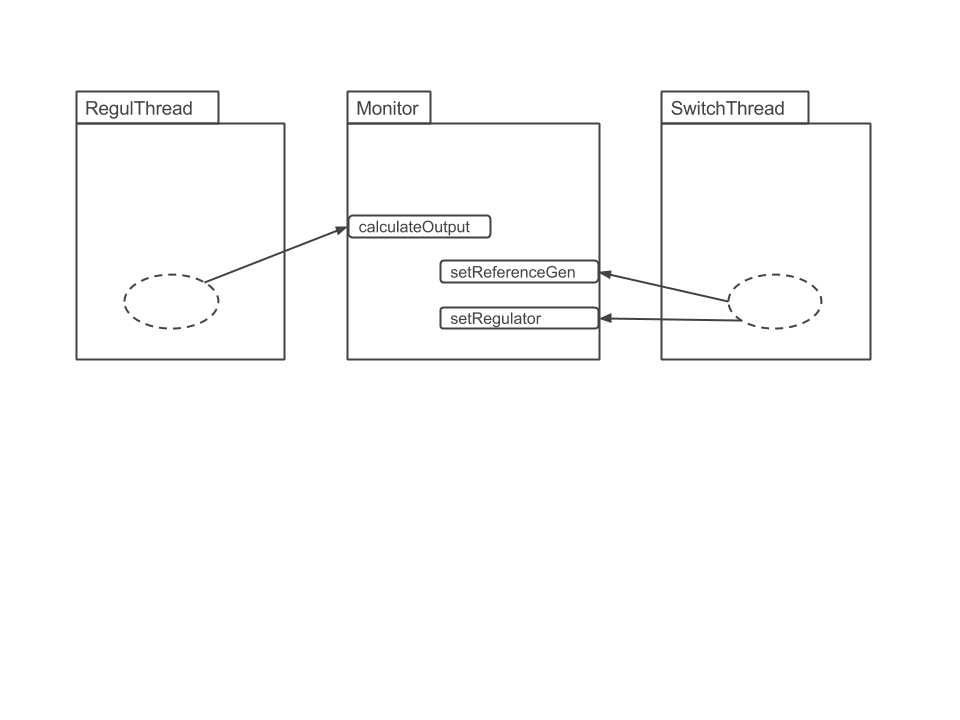
\includegraphics[width=0.8\textwidth]{figures/Overall.png}
\caption{Abstracted UML of the code structure only showing the two threads involved in control and the  monitor. The name of the methods are not the same as in the actual code. The helper classes they use in doing their
task are for readability reasons not shown but are described in detail in the subsections of this chapter.}
\label{overall_fig}
\end{figure}

\subsubsection{Main.java}
%behöver nog inte beskrivas så ingående

\subsection{Threads}

\subsubsection{RegulThread.java}

\subsubsection{SwitchThread.java}

\subsection{Checker classes}
Checker classes provide a method to determine if a state is "OK" in some way. We use this to find out when we should continue to the next part of the catch-throw sequence. These classes are found in the \texttt{checker} package.
\subsubsection{StateChecker.java}
\texttt{StateChecker} is the abstract superclass of all the checkers. It has two methods.

The method \texttt{check(double[])} receives our measured values and returns a boolean describing if the state of the system fulfills some condition, depending on the implementation in subclasses.

\texttt{reset()} is used when activating a checker to reset their internal states, so any previous usage of the object won't  affect the current workings. This method will be empty in subclasses that have no internal state.

%\subsubsection{BallOnBeamChecker.java}
%just nu använder vi inte den här, men det finns förändringar vi kan göra för att den ska funka

\subsubsection{ConstBallChecker.java}

This subclass checks if a ball has been around a specified point on the beam for a sufficient number of samples in a row. It provides the method \texttt{setValue(double)} for choosing the wanted stationary point.

\subsubsection{ConstBeamChecker.java}

Exactly the same as \texttt{ConstBallChecker}, except for the angle of the beam.

\subsubsection{LEDChecker.java}

Checks if the beam is in the pickup position - in other words if the LED is on. This is done by actually reading the digital in channel.

\subsection{Regulator classes}

\subsection{Reference generator classes}

\subsection{Miscellaneous classes} 	%Beskrivning av klasser som inte passar in under andra rubriker, tex Main och OpCom
%tror även Monitor bör få en snabb beskrivning här, men de flesta metoder i monitorn bör förklaras i beskrivningen av de klasser som faktiskt använder dem.




